%% 
%% Copyright 2007, 2008, 2009 Elsevier Ltd
%% 
%% This file is part of the 'Elsarticle Bundle'.
%% ---------------------------------------------
%% 
%% It may be distributed under the conditions of the LaTeX Project Public
%% License, either version 1.2 of this license or (at your option) any
%% later version.  The latest version of this license is in
%%    http://www.latex-project.org/lppl.txt
%% and version 1.2 or later is part of all distributions of LaTeX
%% version 1999/12/01 or later.
%% 
%% The list of all files belonging to the 'Elsarticle Bundle' is
%% given in the file `manifest.txt'.
%% 

%% Template article for Elsevier's document class `elsarticle'
%% with numbered style bibliographic references
%% SP 2008/03/01

\documentclass[preprint,12pt]{elsarticle}

%% Use the option review to obtain double line spacing
%% \documentclass[authoryear,preprint,review,12pt]{elsarticle}

%% Use the options 1p,twocolumn; 3p; 3p,twocolumn; 5p; or 5p,twocolumn
%% for a journal layout:
%% \documentclass[final,1p,times]{elsarticle}
%% \documentclass[final,1p,times,twocolumn]{elsarticle}
%% \documentclass[final,3p,times]{elsarticle}
%% \documentclass[final,3p,times,twocolumn]{elsarticle}
%% \documentclass[final,5p,times]{elsarticle}
%% \documentclass[final,5p,times,twocolumn]{elsarticle}

%% For including figures, graphicx.sty has been loaded in
%% elsarticle.cls. If you prefer to use the old commands
%% please give \usepackage{epsfig}

%% The amssymb package provides various useful mathematical symbols
\usepackage{xspace}
\usepackage{amssymb}
\usepackage{subcaption}
\usepackage[printonlyused]{acronym}
%%
\acrodef{AHB}[AHB-PNW]{Advanced Hardwood Biofuels Northwest}
\acrodef{BCAM}{Bioenergy Crop Adoption Model} 
\acrodef{CCSM3}{Community Climate System Model version 3}
\acrodef{CDL}{Cropland Data Layer}
\acrodef{GBSM}{Geospatial Bioenergy Systems Model}
\acrodef{GIS}{Geographical Information System}
\acrodef{IPCC}{Intergovernmental Panel on Climate Change}
\acrodef{mmu}{minimum mapping unit}
\acrodef{NASS}{National Agricultural Statistics Service}
\acrodef{NLCD}{National Land Cover Dataset}
\acrodef{NRCS}{Natural Resources Conservation Service, Department of Agriculture}
\acrodef{NREL}{National Renewable Energy Laboratory}
\acrodef{PNW}{Pacific Northwest}
\acrodef{PRISM}{Parameter-elevation Relationships on Independent Slopes Model} 
\acrodef{SRWC}{short rotation woody crops}
\acrodef{STATSGO}{State Soil Geographic}
\acrodef{USGS}{United States Geological Survey}
\acrodef{SECRETS}{Stand to Ecosystem CaRbon and EvapoTranspiration
Simulator}
%% 3PG acronyms
\acrodef{3pg}[\textsc{3PG}]{Physiological Principles in Predicting Growth}
\acrodef{BLcond}[\ensuremath{BL_{cond}}]{Boundary layer conductance}
\acrodef{dbh}[\ensuremath{dbh}]{Diameter at Breast Height}
\acrodef{DOB}[\ensuremath{DOB}]{Basal Diameter}
\acrodef{LAIt}[\ensuremath{LAI_{T}}]{Target Leaf Area Index}
\acrodef{LAI}[\ensuremath{LAI}]{Leaf Area Index}
\acrodef{NPPdef}[\ensuremath{NPP_{def}}]{$NPP$ deficit}
\acrodef{NPPt}[\ensuremath{NPP_{T}}]{Target Productivity}
\acrodef{NPP}[\ensuremath{NPP}]{Net Primary Productivity}
\acrodef{RP}[\ensuremath{RP}]{Root Productivity}
\acrodef{Rdp}[\ensuremath{R_{\Delta}}]{monthly root contribution}
\acrodef{Re}[\ensuremath{e_{R}}]{root conversion efficiency}
\acrodef{SLA}[\ensuremath{SLA}]{Specific Leaf Area}
\acrodef{WF}[\ensuremath{W_F}]{Foliage biomass}
\acrodef{WS}[\ensuremath{W_S}]{Stem biomass}
\acrodef{WR}[\ensuremath{W_R}]{Root biomass}
\acrodef{W}[\ensuremath{W}]{Plant biomass}
\acrodef{dRres}[\ensuremath{\Delta R_{res}}]{Residual root contribution}
\acrodef{dW}[\ensuremath{\Delta W}]{Total Monthly Growth}
\acrodef{fSW}[\ensuremath{f_\Theta}]{soil water limiter}
\acrodef{fAge}[\ensuremath{f_{age}}]{age growth limiter}
\acrodef{fNutr}[\ensuremath{f_{nutr}}]{nutritional limiter}
\acrodef{fT}[\ensuremath{f_T}]{temperature limiter}
\acrodef{fi}[\ensuremath{f_i}]{Generic growth limiters}
\acrodef{k}[\ensuremath{k}]{radiation extinction coefficient}
\acrodef{lf}[\ensuremath{lf}]{Litter fall}
\acrodef{pRx}[\ensuremath{x_{pR}}]{maximum root fraction}
\acrodef{pR}[\ensuremath{p_R}]{Root allocation}
\acrodef{pfs}[\ensuremath{p_{FS}}]{foliage to stem allocation fraction}
\acrodef{VI}[\ensuremath{VI}]{Volume Index}
\acrodef{sps}[\ensuremath{n_{stems}}]{Stems per stump}
\acrodef{cancover}[\ensuremath{CanCover}]{canopy coverage}
\acrodef{LA}[\ensuremath{LA}]{Leaf Area per stem}
\acrodef{swc}[\ensuremath{\Theta_{c}}]{$f_\Theta$ constant}
\acrodef{swp}[\ensuremath{\Theta_{P}}]{$f_\Theta$ power}
\acrodef{maxAWS}[\ensuremath{S_x}]{Maximum available soil water}
\acrodef{AWS}[\ensuremath{S}]{Available soil water}

% Tests
%\acrodef{HW1}{}
%\acrodef{HW2}{Hardwood Default in Coppice}

%\newcommand{\degree}{\ensuremath{{}^{\circ}}\xspace}
\newcommand{\degree}{\ensuremath{{}^{\circ}}\xspace}

%% The amsthm package provides extended theorem environments
%% \usepackage{amsthm}

%% The lineno packages adds line numbers. Start line numbering with
%% \begin{linenumbers}, end it with \end{linenumbers}. Or switch it on
%% for the whole article with \linenumbers.
%% \usepackage{lineno}

\journal{Biomass \& Bioenergy}

\begin{document}

\begin{frontmatter}

%% Title, authors and addresses

%% use the tnoteref command within \title for footnotes;
%% use the tnotetext command for theassociated footnote;
%% use the fnref command within \author or \address for footnotes;
%% use the fntext command for theassociated footnote;
%% use the corref command within \author for corresponding author footnotes;
%% use the cortext command for theassociated footnote;
%% use the ead command for the email address,
%% and the form \ead[url] for the home page:
%% \title{Title\tnoteref{label1}}
%% \tnotetext[label1]{}
%% \author{Name\corref{cor1}\fnref{label2}}
%% \ead{email address}
%% \ead[url]{home page}
%% \fntext[label2]{}
%% \cortext[cor1]{}
%% \address{Address\fnref{label3}}
%% \fntext[label3]{}

\title{Modeling Poplar Growth as a Short Rotation Woody Crop for Biofuels in the Pacific Northwest}

%% use optional labels to link authors explicitly to addresses:
%% \author[label1,label2]{}
%% \address[label1]{}
%% \address[label2]{}

\author[lawr]{Q. J. Hart}
%\author[en]{N. C. Parker}
%\author[plant]{B.L. Yeo}
\author[en]{V. Bandaru}
%\author[lawr]{J. R. Merz}
\author[bioag]{B. M. Jenkins}

\address{Department of Land, Air, and Water, University of California, Davis, USA\fnref{lawr}}
%\address{Department of Plant Sciences, University of California, Davis, USA\fnref{plant}}
\address{Energy Institute, University of California, Davis, USA\fnref{en}}
\address{Department of Biological and Agricultural Engineering, University of California, Davis, USA\fnref{bioag}}

\begin{abstract}
%% Text of abstract
  The \acf{AHB} is a consortium of university and industry partners
  investigating the development of a sustainable hardwood biofuels
  industry in Washington, Oregon, Northern California and Northern
  Idaho in the U.S.  Inspired in part by the U.S. Energy Independence
  and Security Act 2022 targets for renewable fuel (renewable fuel
  standard), \ac{AHB} is carrying out research and development to
  support a system for growing and converting hardwoods, such as
  hybrid poplars, into liquid biofuels that are fully compatible with
  existing infrastructure.

  Predicting the economic viability and environmental sustainability
  of a biofuels industry based on this feedstock requires spatial
  predictions of the growth and yield of \acf{SWRC} under various
  environmental conditions and throughout the entire Pacific Northwest
  region.  The \acf{3pg} model was selected and modified for \ac{SRWC},
  particularly for poplar plantation methodologies.  This included
  developing a sub-model which takes into account the coppicing
  strategy for harvesting poplar.

  A physiological growth model such as \ac{3pg} is advantageous because it
  allows variation of growth parameters and assumptions regarding
  management practices for poplar species.  Because it is a canopy
  carbon balance model, allocations for both above and below ground
  biomass can be tracked for life-cycle analysis of the product fuels.

  The original \ac{3pg} model does not include coppicing as a management
  practice, which is problematic as it cannot reasonably account for
  post-coppicing regrowth.  The extended model includes coppicing with
  a general model that allows a monthly growth contribution from an
  existing root mass.  The model specifies a relatively small
  contribution of aboveground growth from the accumulated root mass
  after coppicing in order to initiate the next cycle of production.

  The \ac{3pg} model was validated against a number of field studies
  related to the growth of poplar as a \ac{SRWC} biofuel feedstock.  The
  parameterized model was then applied to the entire Pacific Northwest
  region, using appropriate climatological and soil input data.
  Climate data included both historical patterns as well as predicted
  patterns from simulations under various climate scenarios.  The
  result was a map of predicted yields and expected bounds on the
  variation of these yields useful for determining when it becomes
  economically feasible for poplar to be grown within the study
  area. Results were integrated with other models that allow for
  optimizing the crop selection and biorefinery site selection.
  Important findings from the model include; validation of the \ac{3pg}
  model for coppiced \ac{SRWC} plantings, estimates of biomass feedstock
  yields under different irrigation patterns and weather conditions,
  and annual estimates for feedstock availability when combined with
  crop adoption scenarios.

\end{abstract}

\begin{keyword}
%% keywords here, in the form: keyword \sep keyword
  Short rotation woody crops \sep Poplar \sep \ac{3pg} \sep Yield
  estimations \sep Pacific Northwest, USA.

%% PACS codes here, in the form: \PACS code \sep code

%% MSC codes here, in the form: \MSC code \sep code
%% or \MSC[2008] code \sep code 

\end{keyword}

\end{frontmatter}

%% \linenumbers

%% main text
\section{Introduction}
\label{sec:introduction}

Using climatological and soil parameters along with the \ac{3pg} forest
growth model, yield predictions for poplar plantations can be made for
the entire Pacific Northwest.  This yield model can be overlaid with
land use patterns to predict yields for potential plantation
locations.  Yield maps are the results of running the \ac{3pg} Model for
the entire \ac{AHB} region. Weather information is derived from the PRISM
Climate Group~\cite{daly2008} and the \acf{NREL} monthly radiation
data (Marion, 1994). Soils data is derived from
\acf{STATSGO}~cite{soil-statsgo2012}.

With appropriate input information, the \ac{3pg} model can predict
yields for the entire Pacific Northwest study region, under various
irrigation scenarios.  When linked with models of crop adoption,
annual feedstock estimates are possible.

For example, a companion model, the \acf{BCAM} predicts price levels
where poplar competes with existing crops in general cropping regions.
The yield results, along with the \ac{BCAM} predictions can be used in
the \acf{GBSM} in order to optimize where in the region poplar might
be adopted.

The current model makes these estimations on an 8x8 km2 grid, a
resolution that is fairly taxing for the solver of the \ac{GBSM}
model.  Subsequent model runs at a finer scale can test the best
scales for application of these models.

\section{Methods and Calculation}

The goal of this study is to create a map of poplar growth potential
for this region that can inform our participants, and subsequent
models on the predicted yields from \ac{SRWC} plantations.

Figure~\ref{fig:grid} shows the study area, the Pacific Northwest of
the United States, incorporating Washington, Oregon, Northern
California, and Western Idaho.  This definition of the Pacific
Northwest is somewhat inclusive in the South, including the northern
part of California.

A regular grid is used to partition the region.  The initial size of
the grid is relatively coarse $8192 \times 8192$ (m x m), and designed
to reduce some of the complexity of our regional optimization models.
The projection is an Albers equal area projection with standard
longitude 120\degree West, and parallels at latitudes 41\degree and
47\degree North~\cite{Butler}. This somewhat specialized projection
insures the pixels maintain a constant area, while maintaining good
conformity for our transportation networks.  The pixel size is
$2^{13}$ (m).  This allows easy scaling up and down of the data to
different resolutions while maintaining common edges.  For example,
the \ac{NLCD} dataset, used in this study, was originally imported at
$2^5$ (m), and scaled upwards to determine percentages of landcover
for each pixel.

\begin{figure}[hp]
  \centering
  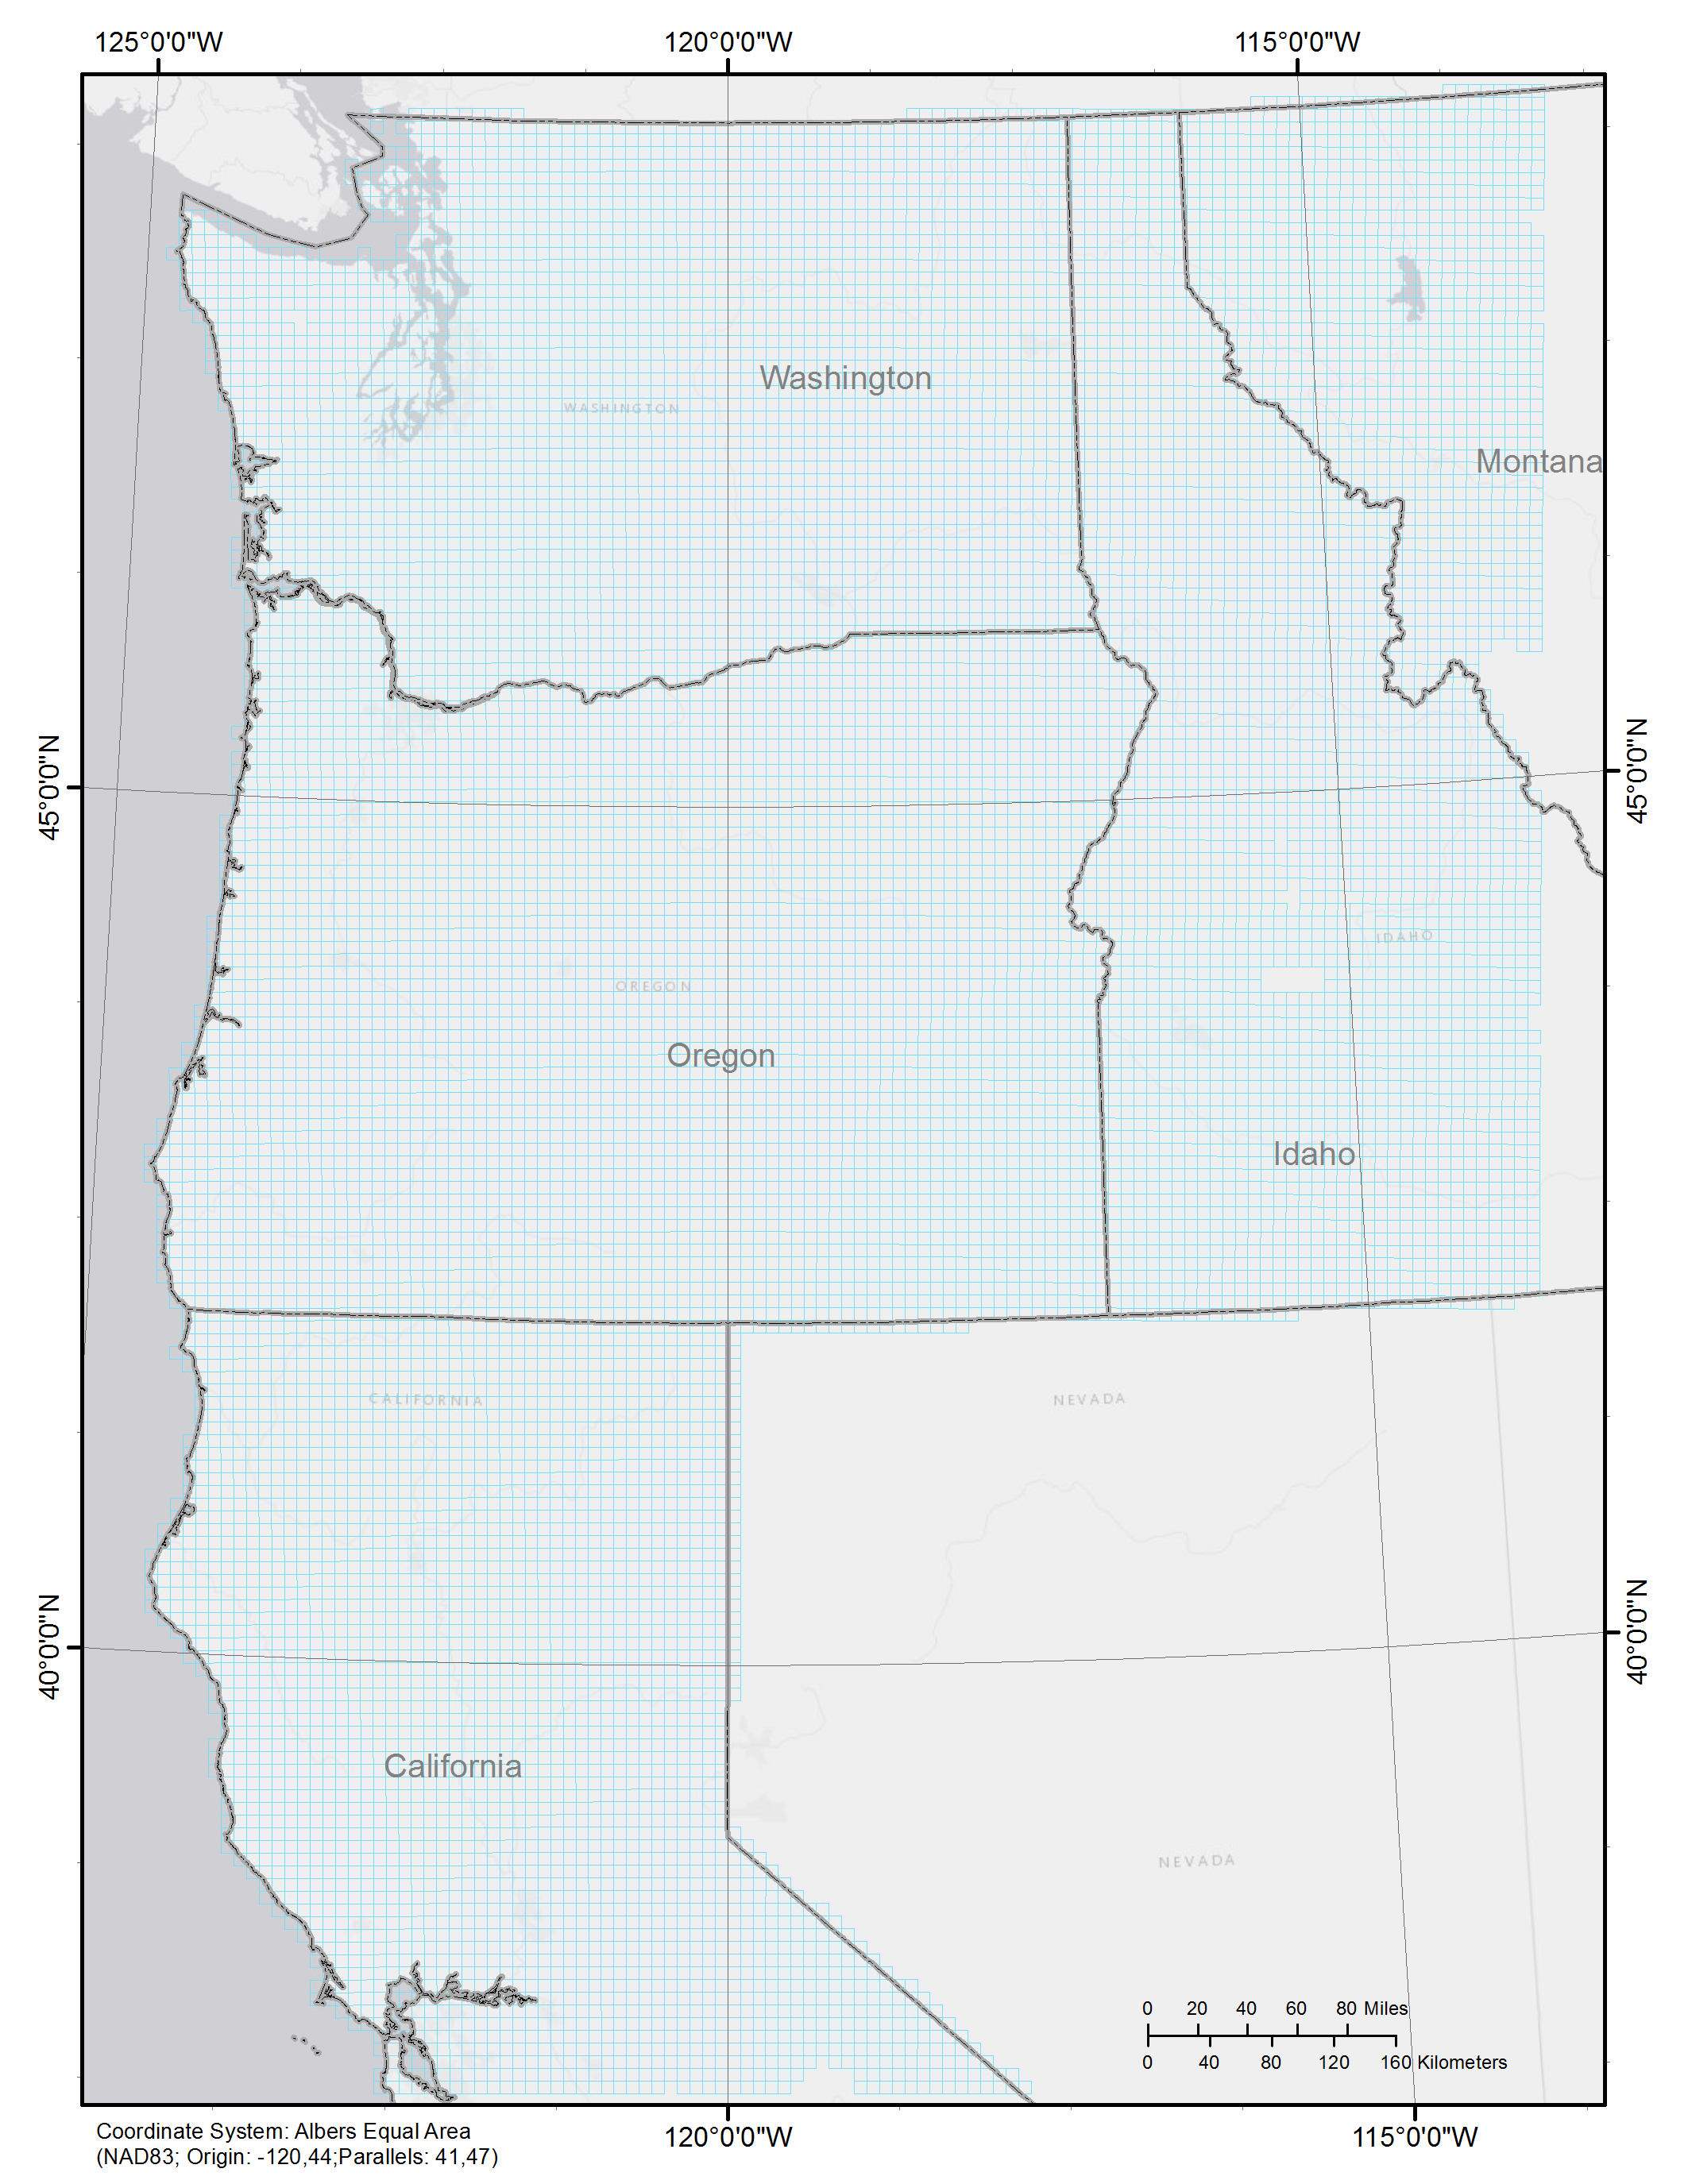
\includegraphics[width=1.0\linewidth]{grid}
  \caption{Location of the study area, with grid layer overlaid.}
  \label{fig:grid}
\end{figure}

Data processing was carried out with a postgresql database, with the
postgis geospatial extensions~\cite{pgsql,Holl2009,postgis}.
Specialized calculations were implemented as postgresql functions, using
various scripting languages; SQL, PLSQL, Javascript, and R.

\begin{table}
  \centering
  \begin{tabular}[hp]{|l|l|}
    \hline
    Parameter & Source(s) \\
    \hline
    Temperature & \acs{PRISM} \\
    Precipitation & \acs{PRISM} \\
    Solar Radiation & \ac{USGS} \\
    \hline
  \end{tabular}
  \caption{Required Model Inputs}
  \label{tab:input}
\end{table}
\subsection{\acs{3pg} Model Formulation}
\label{sec:3pg}

The \acf{3pg} model~\cite{Landsberg1997, landsberg2010physiological,
  Sands2004} takes as inputs weather data, and site factors, including
soil parameters, initial stocking conditions, management practices,
and species definitions.  In this study, the \ac{3pg} model is run at
a monthly timestep. At each step the physiological parameters are
calculated and carried forward to the next month.  These incremental
physiological parameters can be plotted to compare model predictions
with field results at multiple stages in the plantation’s history.
Figure~\ref{fig:overview} gives an overview of the \acf{3pg} model.

\begin{figure}[p]
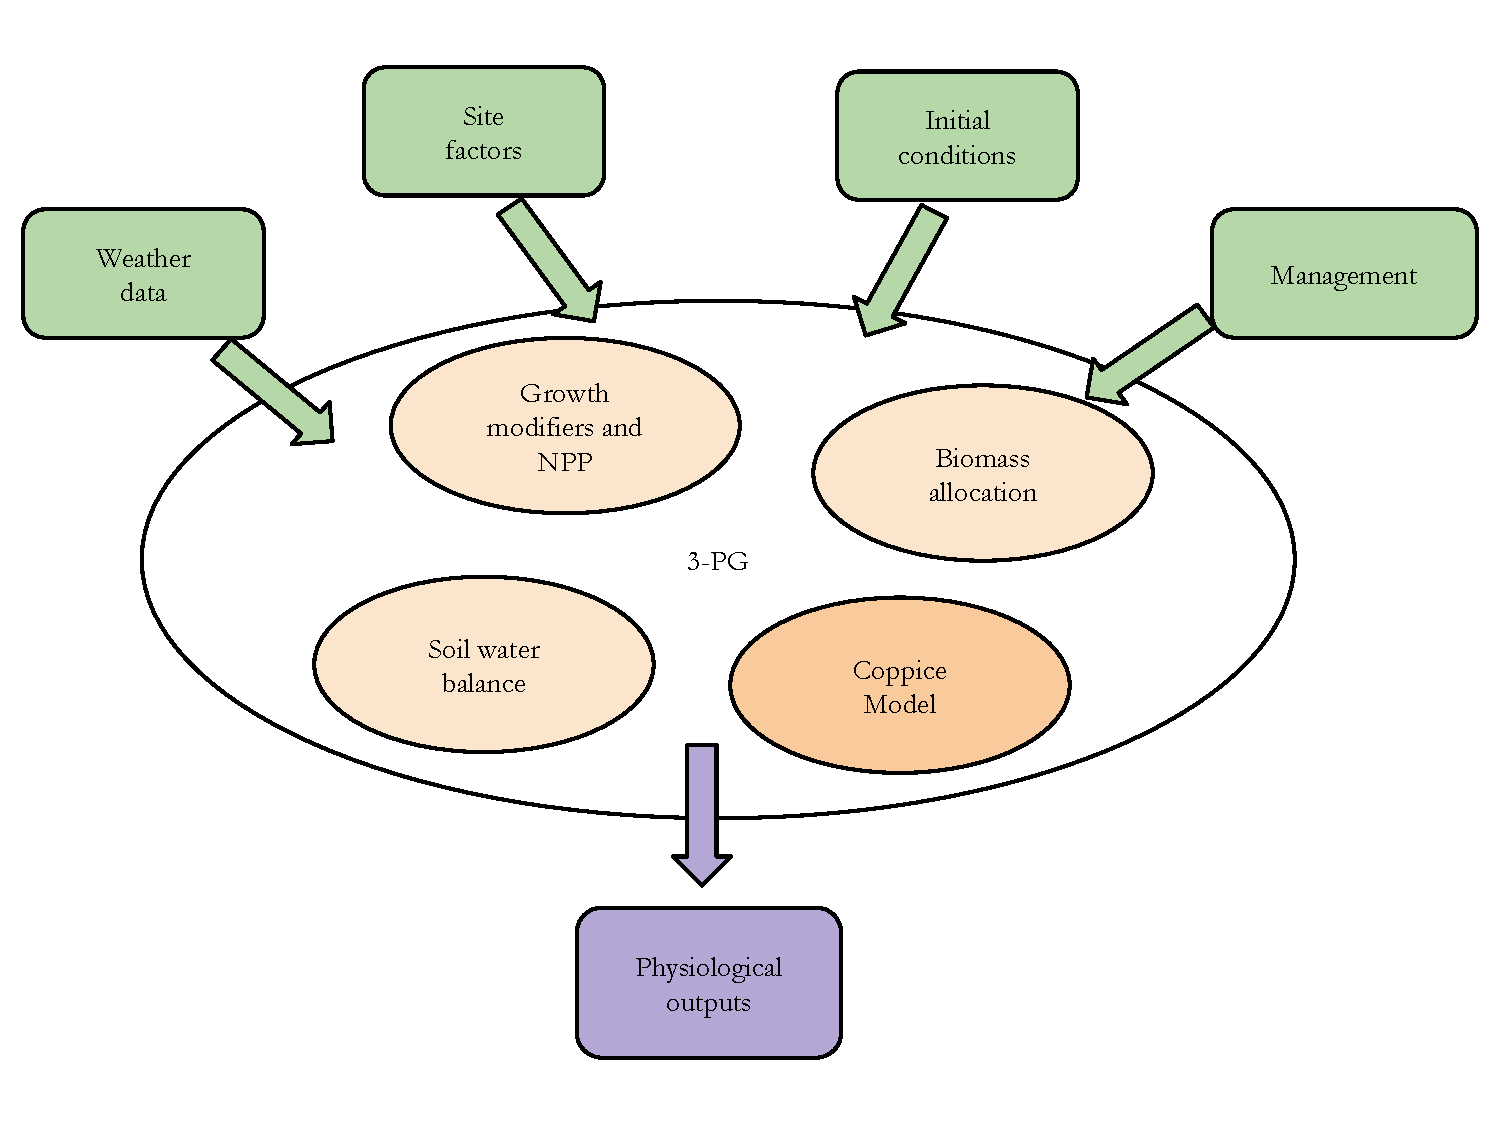
\includegraphics[width=\linewidth]{model_overview}
\caption{ The \ac{3pg} model's main inputs.  Running at a monthly timestep, with
appropriate input parameters, the model predicts tree growth and a
number of other parameters.}
\label{fig:overview}
\end{figure}

The original \ac{3pg} model allocates mass produced from transpiration
into the the creation of new roots, stems and foliage.  After
coppicing however, the model has no mechanism to increase start of
re-growth from the root.  A simple coppicing model has been developed
to add an additional production from the root system after
coppicing\cite{hart14-coppice}.  The seasonal timing of the
contribution is moderated by comparing the actual \ac{NPP} to the
\ac{NPP} the root could produce if it had a more complete canopy.
This difference serves as a target for the root contribution.  This
method times regrowth with climatic conditions that are favorable for
growth.  The monthly root contribution affects the length of time for
the contribution to be made.  In poplar plantations, the initial
planting is modeled the same way, however with different parameters to
model initial propagation methods.

In order to calculate the t

\subsubsection{Climatic and Radiation Data}
\label{sec:climate}

%http://cses.washington.edu/cig/pnwc/pnwc.shtml
%http://en.wikipedia.org/wiki/Climate_of_California

The Pacific Northwest weather patterns are influenced primarily by the
Pacific storm track, which brings in the bulk of precipitation in the
months of October through March, and the location and size of the
mountain ranges, which moderate both the precipitation, and the
temperatures throughout the year.

In order to predict temperatures and precipitation on the near term,
the \acf{PRISM} dataset was used.  \ac{PRISM} extrapolates station
data spatially to a uniform grid using weights derived from the
physiographic similarity of the station to the grid cell. These
similarity measures include location, elevation, coastal proximity,
topographic facet orientation, vertical atmospheric layer, topographic
position, and orographic effectiveness of the terrain.  \ac{PRISM}
data is available on a 2.5 minute geographic grid.

16 years of \ac{PRISM} data were interpolated (cubic spline) to the
\ac{AHB} grid averaged to determine a representative weather pattern
used near term modeling for the \ac{AHB} yield predictions.
Figure~\ref{fig:temp} show annual mean temperature and precipitation
variation of the region.  Isolines show the standard deviation between
annual mean temperature to the monthly mean temperature.  Similarly
isolines are shown on the precipitation map.

\begin{figure}[hp]
  \centering  
  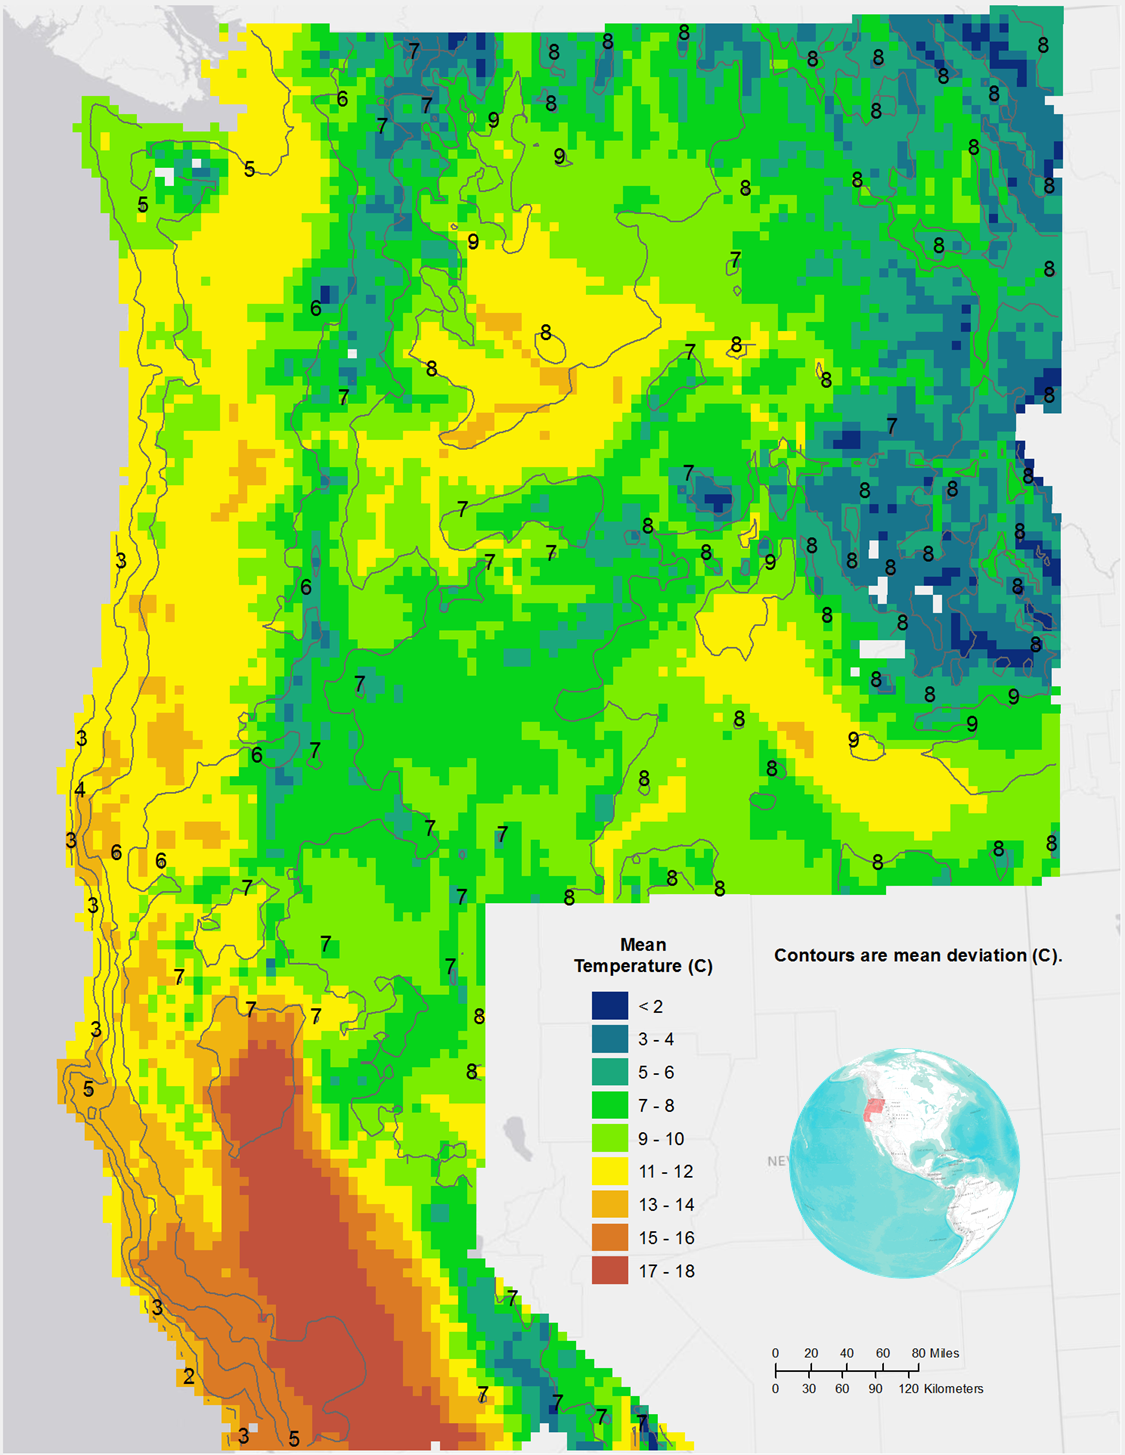
\includegraphics[width=1\linewidth]{dailytemp}  
  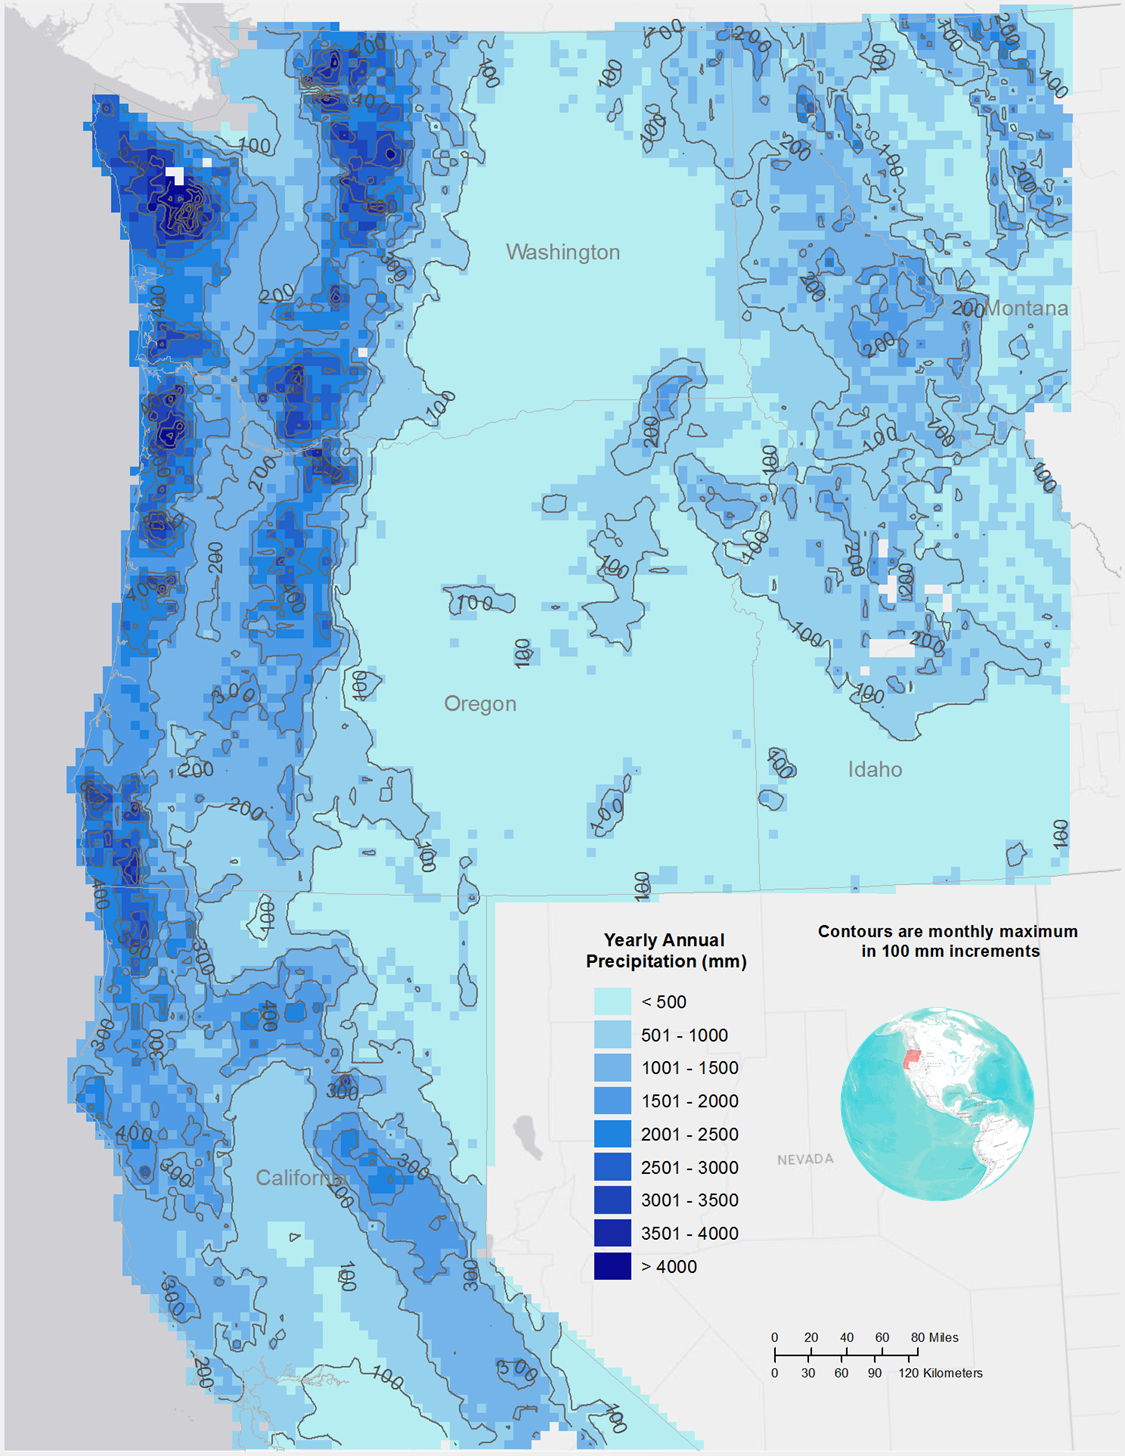
\includegraphics[width=0.45\linewidth]{precip}  
\caption{Mean annual Temperature, with isolines showing the standard deviation in monthly temperature.}
  \label{fig:temp}
\end{figure}

\begin{figure}[hp]
  \centering  
  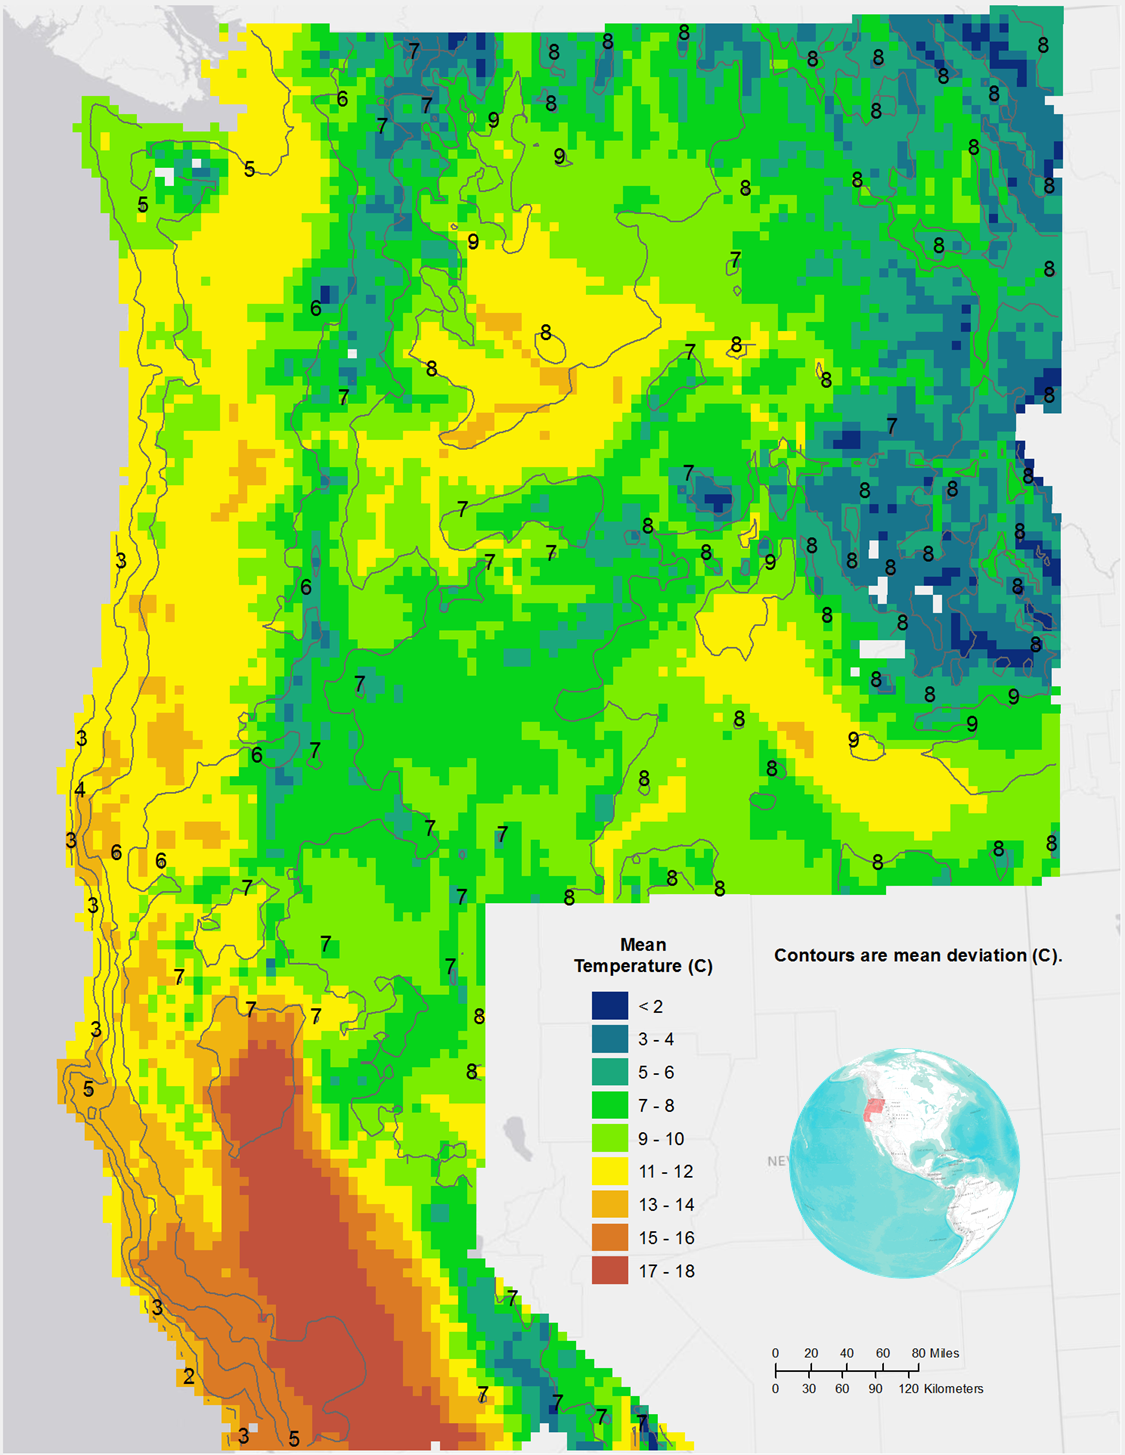
\includegraphics[width=0.45\linewidth]{dailytemp}  
  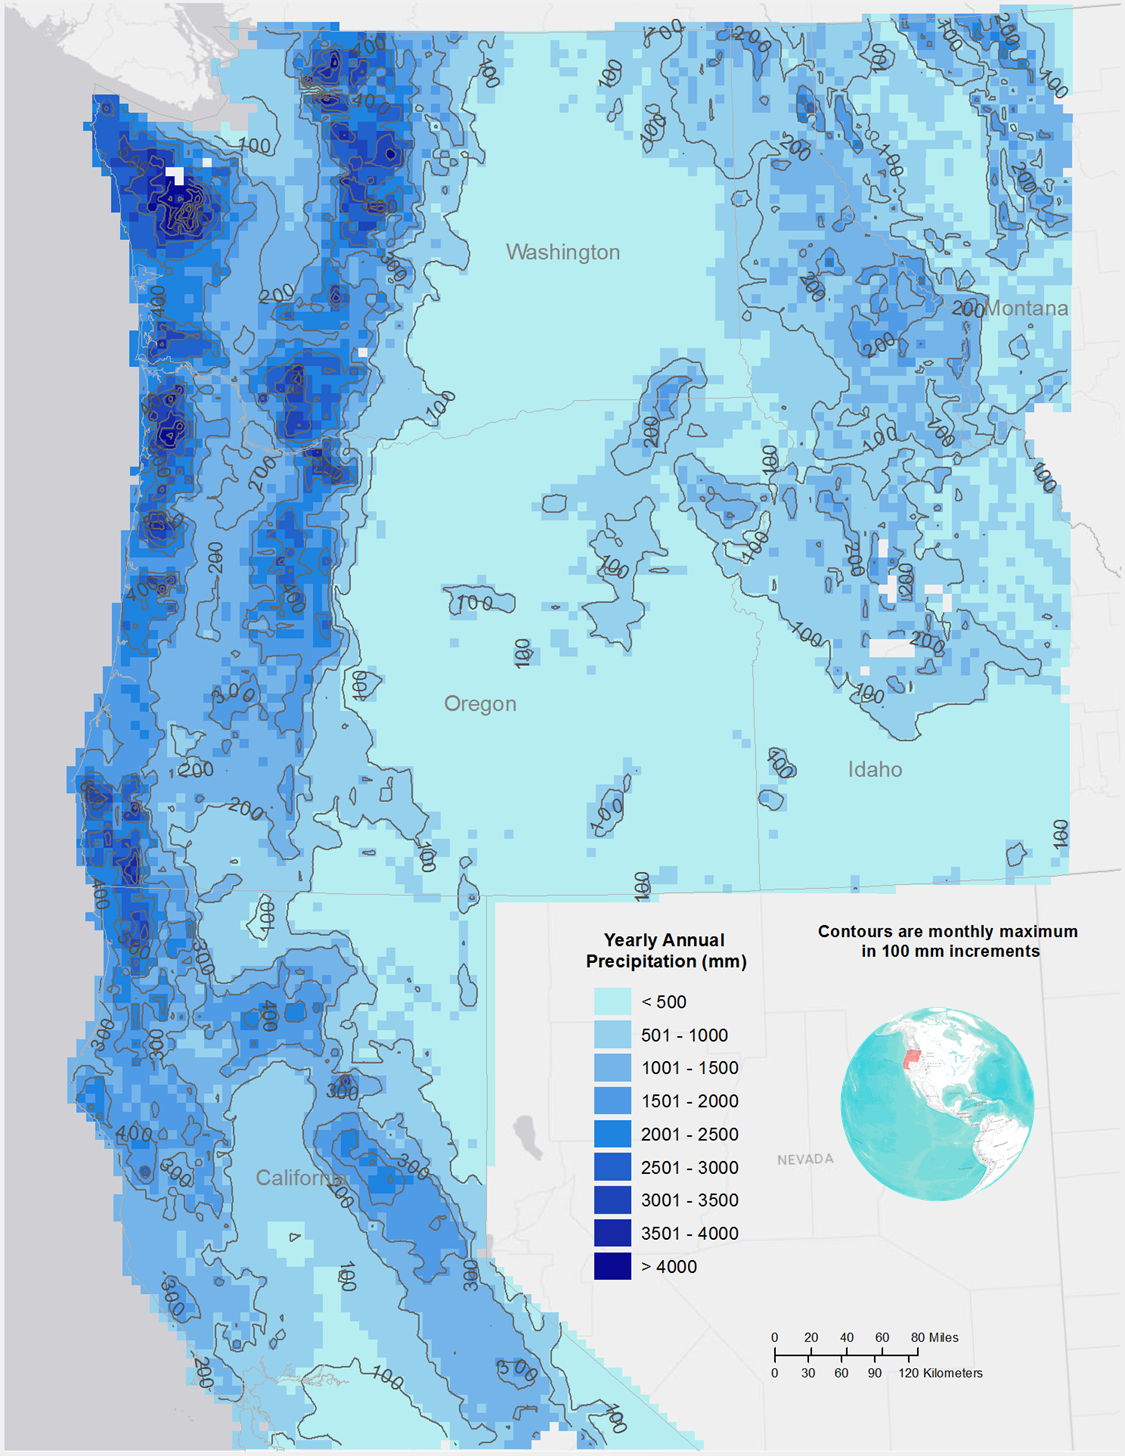
\includegraphics[width=0.45\linewidth]{precip}  
\caption{Total annual rainfall maps, with iso lines showing the maximum monthly rainfall.}
  \label{fig:temp}
\end{figure}

\subsubsection{Soil Parameters}
\label{sec:soil}

\ac{3pg} uses a single layer soil model that maintains an estimate of
the amount of water available at any timestep in the model.  In
addition, \ac{3pg} includes a growth limiter related to the available
water in the soil, and the soil type.  These require a number of soil
parameters.  \ac{maxAWS} determines the maximum holding capacity of
the soil.  The limiter \ac{fSW} is parameterized with two values,
$\acs{fSW} = \frac{1-(1-\acs{AWS}/\acs{maxAWS})^{\acs{swp}}}{1+((1-\acs{AWS}/\acs{maxAWS})/\acs{swc})^{\acs{swp}}}$, 
where \ac{swp} and \ac{swc} are functions of the soil type.

These parameters are all determined using the \ac{STATSGO} database.
\ac{STATSGO} is a national soil database, distributed by the
\ac{NRCS}.  \ac{STATSGO} maps are designed for regional studies, and
the soil inventories are typically generalized from more detailed
surveys, or from a combination of ancillary datasets.  Individual
\ac{STATSGO} areas can contain multiple soil components, and the map
units are linked to attributes the soil data base which gives the
proportionate extent of the component soils and their associated
properties.  The \ac{mmu} is about 625 (ha).  For each pixel in the
modeling grid, intersecting map units are averaged for the estimated
pixel values.  1887 different soil were used, contributing anywhere
from 144 to 1.3M (ha).

\ac{maxAWS} is directly taken from the \ac{STATSGO} database which
Figure~\ref{fig:aws} shows the \ac{maxAWS} estimates.

Included in the figure are the lines designating the soil polygons
used.  

\ac{swp} and \ac{swc} 

\begin{figure}
  \centering
  
  \caption{\ac{STATSGO} derived maximum available water estimates. }
  \label{fig:aws}
\end{figure}


\subsection{Land Classification and Irrigation}
\label{sec:land}

Available climatic data makes it possible to make estimations for
Poplar growth throughout the \ac{PNW} region.  This may provide
interesting comparisons of changes in yield, but is not very suitable
for determining regional trends, as not all lands are equally likely
to be available for Poplar plantations.  Variables like land
ownership, topography and salinity, influence the technical capability
of growing Poplar.  

In addition, the ability to irrigate a poplar plantation can have
large effects on the predicted yields of poplar.  Determining which
areas in the \ac{PNW} region are liable to be available for irrigation
can significantly influence regional polar harvest estimations.  



\begin{figure}[hp]
  \centering
  
  \caption{Land Classification}
  \label{fig:land}
\end{figure}

\subsection{Climate Change}
\label{sec:climate}

Three different climate change scenarios were tested; AB1: foo, B2:
bar, and DF: fubar.  These represent some of the more commonly used
IPCC climate change scenarios.  Estimations of the expected change in
climate came from the IPCC ensemble estimations~\cite{ipcc-ensemble}.
These estimations are an amalgamation of 32 different climate change
scenarios.  The ensemble predictions are available at 0.5 minute grid
cells.  Estimations of change in the next fifty years were used in
these climate change estimations.

The \ac{IPCC} estimations cannot be used directly, especially
comparitively to the the current estimations using the \ac{PRISM}
data.  This is because when comparing the \ac{IPCC}'s somewhat coarse
scale estimations, to the more detailed \ac{PRISM} estimations the
current (2000-2014) predictions exhibit bias in their estimations.
Therefore, the \ac{IPCC} estimations were used to determine the
predicted change in temperature and precipitation for the \ac {AHB}
region, and these changes were then applied to the current \ac{PRISM}
estimations. For example, the 50 year change in temperature, and
precipitation for the \ac{FOO} \ac{IPCC} scenario shows a mean
increase in temperature of about ? degrees Celcius, with larger
changes in the foo and the bar.  Mean annual precipitation throughout
the region stays relatively constant, but shows modfications in both
location, and timing of the precipitation do undergo
changes~(Figure~\cite{fig:new-temp}).

\begin{figure}[hp]
  \centering
  
  \caption{Predicted changes in temperature, precipitation }
  \label{fig:new-temp}
\end{figure}

In total, the three \ac{IPCC} scenarios were compared at three
distinct initial planting dates; 2020, 2040 and 2060, and under the
same set of 8 different \ac{3pg} poplar parameterizations, for a total
of 79 estimations per pixel in the \ac{AHB} region.  

\section{Results and Discussion}

\subsection{Poplar Yields}
\label{sec:yield}

\begin{figure}[hp]
  \centering
  
  \caption{Example Poplar growth predictions}
  \label{fig:examples}
\end{figure}

% \subsection{Average Weather patterns}
% Compare the yield from the AVERAGE weather to the yield from the ACTUAL last 16 years of data.

% \subsection{Poplar Crop Adoption}
% \label{sec:bcam-out}

% \begin{table}[hp]
%   \centering
%   \begin{tabular}{|l|c|c|}
    
%   \end{tabular}
%   \caption{Potential Poplar Amounts}
%   \label{tab:potential}
% \end{table}

\subsection{Climate Change}
\label{sec:climate-change}


\begin{table}[hp]
  \centering
  \begin{tabular}{|l|c|c|c|}
    \hline
    Scenario & 2020-2038 & 2040-2058 & 2060-2078 \\
    \hline
    \ac{AB1} & 1 & 2 & 3 \\
    \ac{AB1} & 1 & 2 & 3 \\
    \ac{AB1} & 1 & 2 & 3 \\
    \hline    
  \end{tabular}
  \caption{Mean annual changes in irrigated Poplar yields  over the entire \ac{AHB} region.  
These yields are the mean annual yield for plantations with 5 coppice events, on three year cycles.
The initial year of the predictions are 2020, 2040, and 2060.}
  \label{tab:potential}
\end{table}

The mean change in yields are not necessarily a good estimation of
local estimations of changes in yield predictions.  Regional changes
in temperature and precipitation induce considerable heterogenity in
the yield change estimations.  Looking again, at \ac{IPCC} scenario
\ac{AB2}, for the 2060-2078 time frame, we see considerable -- blah
blah blah -.  These patterns are somewhat similar to all \ac{IPCC}
scenarios, becoming more pronounced as the estimation is moved into
the future~(Figure~\cite{fig:new-change}.

\begin{figure}[hp]
  \centering
  
  \caption{Changes in predicted yield for \ac{IPCC} scenario \ac{AB1}
    for a plantation planting in 2060-2078.}
  \label{fig:land}
\end{figure}

Such estimations can inform both the individual farmer in terms of
predicting long term viability of Poplar plantations as a \ac{SRWC}
feedstock, as well as regional estimations on the mid-term ability of
such a feedstock to provide an expected harvest, and therefore an
expected level of biofuel production.  Not only changes in expected
overall yields, but changes in the spatial distribution of the yields
can have impacts on economic analysis of a \sc{SRWC} based biofuel
industry in the \ac{PNW}.  

Next Steps 

- For irrigated land, Current yields are input into a \ac{BCAM} model
where they compete with existing crops to determine there economic
viability.  It's hard to add water into the system as a direct cost of
operation, because it's a confusing mush of real costs; availability
and rights.  One way to address this issue is to include water as a
zero-sum game in the adoption model.

- For non-irrigated land, marginal and under utilized lands can be
added into the overall agricultural economy as newly minted lands.
These may compete with other agriculture crops, but they can also 

\section{Conclusions}
\label{sec:conclude}

Yields provide viability
Yields help farmers make decisions

TODO
- Look at more localized estimations
- Compare mean estimations to changes in yield based on actual more changing weather patterns
- - IN that same context, look at different time frames for your estimations. 
- - These can provide some larger error bounds on our 



%% The Appendices part is started with the command \appendix;
%% appendix sections are then done as normal sections
%% \appendix

%% \section{}
%% \label{}

%% If you have bibdatabase file and want bibtex to generate the
%% bibitems, please use
%%
\bibliographystyle{elsarticle-num} 
\bibliography{ahb-pnw}

%% else use the following coding to input the bibitems directly in the
%% TeX file.

% \begin{thebibliography}{00}

% %% \bibitem{label}
% %% Text of bibliographic item

% \bibitem{}

% \end{thebibliography}

\end{document}
\endinput
%%
%% End of file `elsarticle-template-num.tex'.

%  LocalWords:  dataset Albers landcover postgresql geospatial SQL
%  LocalWords:  postgis PLSQL Javascript timestep coppicing datasets
